\documentclass[a4paper,12pt]{article} %article, report, book,...


\usepackage{authblk}
\usepackage{xcolor}
\usepackage{graphicx}
\usepackage[round]{natbib}

\begin{document}
\title{My first \LaTeX{} document}
\author[1]{F. Batsleer}
\affil[1]{Terrestrial Ecology Unit}
\date{\today}
\maketitle


%\clearpage

\tableofcontents
\clearpage

My first \LaTeX{} document! Yeay!\\
\section{Introduction}
\textit{\textbf{This will be the intro}}
\subsection{First part of introduction}
\clearpage

\section{Typesetting}
\subsection{Exercise 2}
This is my {\huge introduction}, I want to tell you something {\tiny really}, {\small really}, really, {\color{red} \Large really} \underline{incredible}.\\
My article is \textsc{amazing}.\\
It's \textbf{great}, just great.\\
\textit{Believe me}, we're going to make the \textsc{\color{green} TEREC} great again!\\

\subsection{Exercise 3}
\begin{enumerate}
	\item Wybouw/Bonte retreat 2024
	\begin{itemize}
		\item Where?
		\begin{itemize}
			\item Near Chimay!
			\item Rue du Calvaire 2, Rance
		\end{itemize}
		\item When?
		\begin{itemize}
			\item Monday 23\textsuperscript{th} to Friday 27\textsuperscript{th} of September
		\end{itemize}
	\end{itemize}
	\item Planned activities
	\begin{itemize}
		\item[$\ast$] Scientific sessions
		\begin{itemize}
			\item[$\rightarrow$] Lab day part 1 \& 2
			\item[$\rightarrow$] This \LaTeX{} coding club!
			\item[$\rightarrow$] ... and much more!
		\end{itemize}
		\item[$\ast$] Fun activities
		\begin{itemize}
			\item[$\rightarrow$] Hiking or Parcours
			\item[$\rightarrow$] Visit to Chimay abbey
			\item[$\rightarrow$] Moth trapping
			\item[$\rightarrow$] Quiz
			\item[$\rightarrow$] ... and much more!
		\end{itemize}
	\end{itemize}
\end{enumerate}

\section{Maths}
\subsection{Exercise 4}
...equation \ref{crazy-formula} was used to calculate this metric.
\begin{equation}\label{crazy-formula}
K = \sum_{i=0}^{i=n}\frac{\sqrt{\alpha}}{\delta_{ij}}
\end{equation}


\section{Tables \& Figures}
\subsection{Exercise 5}
\begin{table}[h]
	\begin{tabular}{l|c c c}
		 & & Year & \\
		 \cline{2-4}
		City & 2006 & 2007 & 2008\\
		\hline
		London & 45.000 & 46.000 & 51.000\\
		Berlin & 35.000 & 33.000 & 30.000\\
		Paris & 50.000 & 51.000 & 52.000\\
	\end{tabular}	
\end{table}

\subsection{Exercise 6}
\begin{figure}[ht]
	\centering
	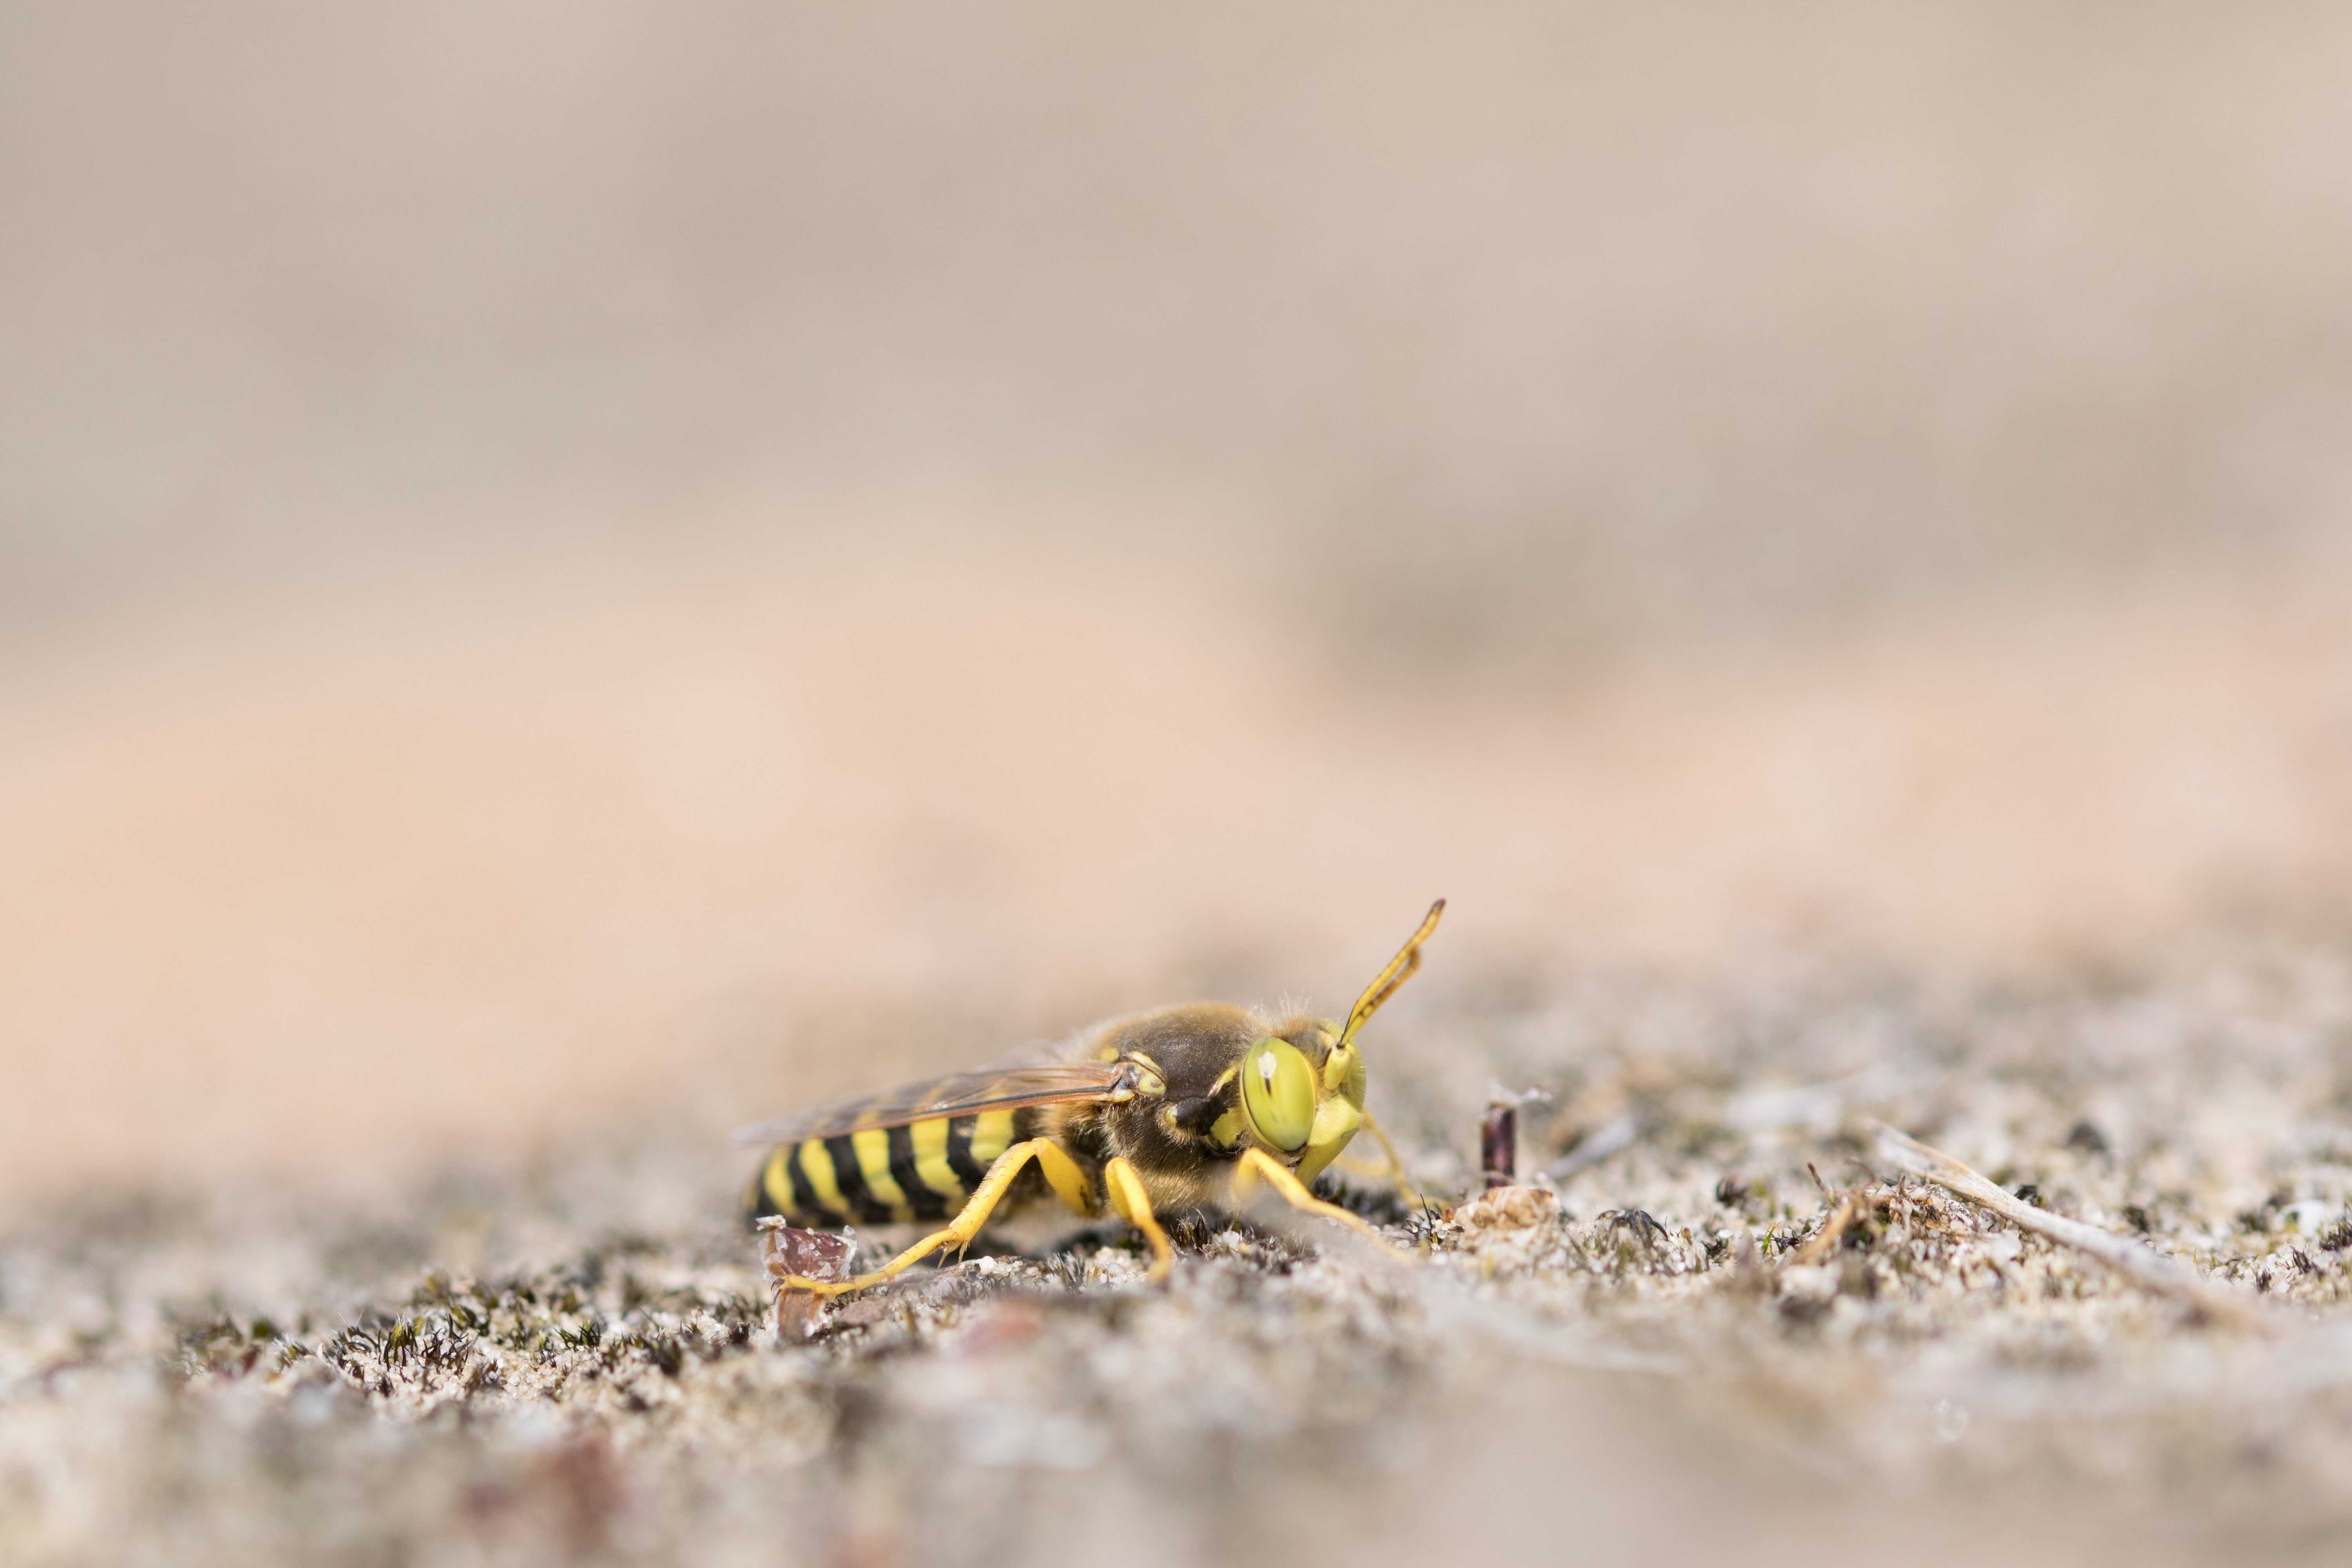
\includegraphics[height=0.5\textwidth]{maleHA.jpg}
	\caption{What an amazing digger wasp!}\label{fig:diggerwasp}
\end{figure}

\section{References}
\subsection{Exercise 7}
\citeauthor{Tengo1996} mention that a digger wasp needs $\pm$ 12 days to finish a nest cycle, provisioning its single larva with flies \citep{Nielsen1945}.

\section{Bibliography}
\bibliographystyle{ecol_let}

\bibliography{ExampleExport}

\end{document}